\subsection{Main results}
\label{sec:results}

\textbf{Rosters.} Three conditions were run over overlapping but non-identical model sets, so we name each
roster explicitly and never write a bare count. The zero-shot leaderboard scored 13 of a pre-registered 14,
with \texttt{moonshotai/kimi-k2.6} unscored under an endpoint-failure gate (no response on a two-structure
$K{=}1$ probe after ten minutes, so the failure is the endpoint rather than the harness); it includes
\texttt{google/gemini-2.5-flash} and not the newer \texttt{gemini-3.6-flash} that heads the ladder, which
is why the leaderboard's best row (0.4429) sits below the ladder's best $R_4$ (0.7333). The image-removal
control attempted 16 and scored 13, with three unscored under a pre-registered 5\% API-error gate. The
coordinate condition attempted 15 and scored 14, with \texttt{qwen/qwen2.5-vl-72b-instruct} unscored for
exceeding both the error and parse gates (34.4\% errors). Every unscored entry is reported unscored rather
than dropped; the per-model roster table is in the supplementary.

The 13 scored zero-shot models ran on the frozen protocol with a verbatim prompt and no per-model tuning
(Figure~\ref{fig:leaderboard}). The best reaches $93/210 = 0.4429$ on the original sample, far below the
oracle's 0.9524.

\begin{figure}[t]
\centering
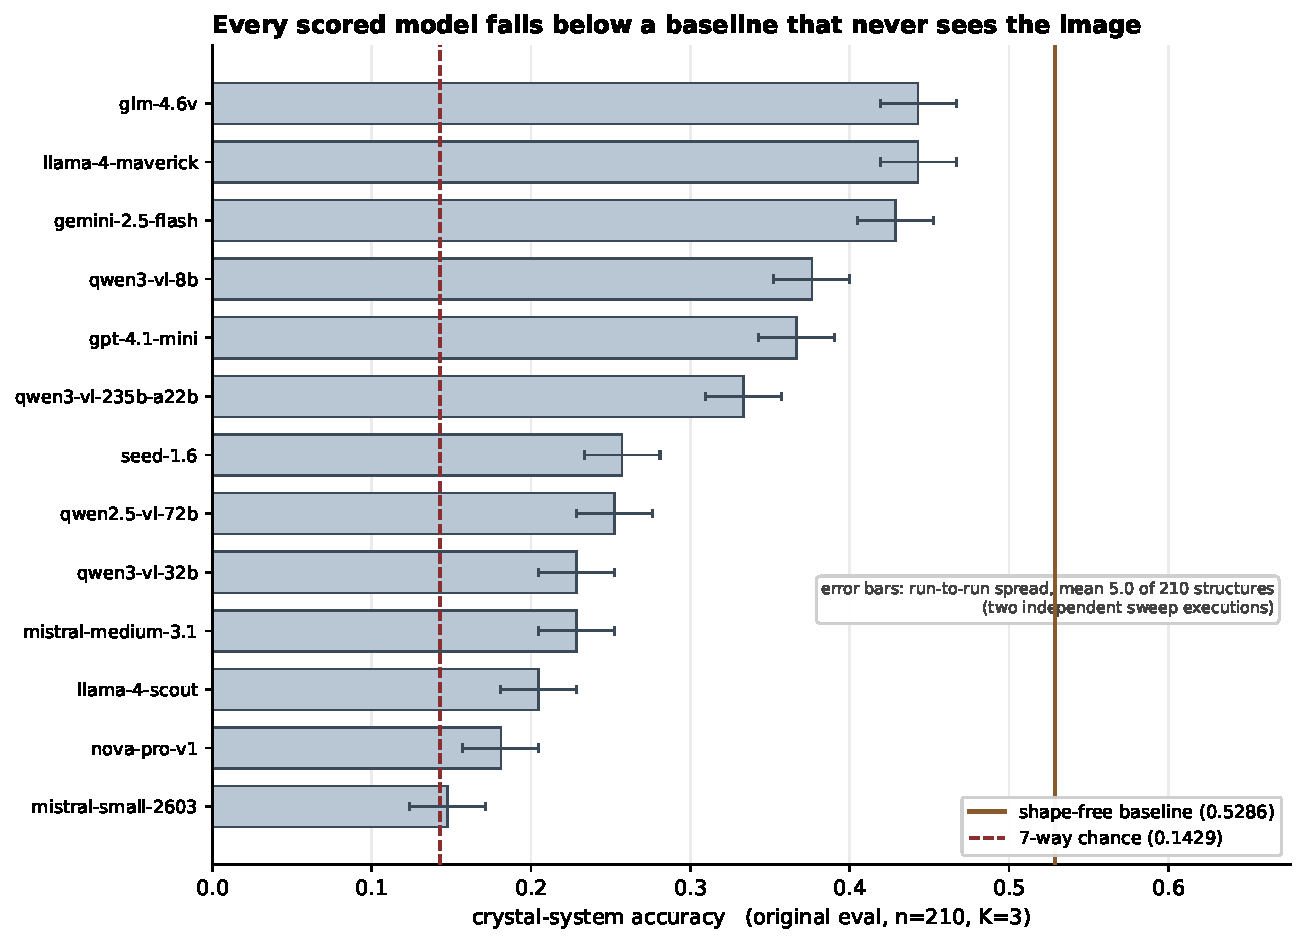
\includegraphics[width=0.8\linewidth]{figures/leaderboard.pdf}
\caption{Zero-shot leaderboard, original sample, $n=210$, $K=3$, 13 scored models across eight vendors.
Dashed line: the shape-free baseline (atom count, density, cell volume) on this sample. Error bars: the
measured run-to-run spread of $K{=}3$ majority voting.}
\label{fig:leaderboard}
\end{figure}

\textbf{A modality-matched reference.} A cell-metric random forest reaches 0.8952 on crystal system, above
every model. This reproduces an established capability rather than contributing one; it is not comparable
to \citet{cryspnet2003}, which predicts symmetry from composition alone, the opposite input and a harder
problem.

\paragraph{The strongest model arm, and what is not claimed for it.}
The 0.6905 figure is a supervised-then-GRPO arm on \texttt{Qwen/Qwen3-VL-8B-Instruct}, reported as a
single-seed point estimate at $K{=}8$; the same adapter gives $139/210 = 0.6619$ at $K{=}3$. It sits inside
the reference arm's across-seed spread ($0.590 / 0.567 / 0.686$), exceeding that arm's best seed by one
structure at $K{=}8$ and trailing it by five at $K{=}3$, so \emph{we make no claim that this arm improves
on the reference arm}. It is used only as the model side of the ceiling-to-model gap (200 against 145,
discordance $61{:}6$, $p = 1.5\times10^{-12}$), which survives any seed in the observed spread. The
three-seed extension was cut; its record and the quantitative argument for the cut are in the
supplementary.
